\chapter{FPS map's representations and features}

In the following chapter we will discuss the genome representation that we have decided to use in order to later evolve maps using a Quality Diversity algorithm. We will discuss two existing genomes, \textit{All-Black} and \textit{Grid-Graph}, and two new genomes that we have introduced, \textit{Point-Line} and \textit{SMT-Genome}. 

Following, we will describe all the features that we have extracted from the maps, divided into \textit{emergent} and \textit{topological}, and how we have calculated them. 

\section{Map representation}
\label{sec:map_genomes}
As discussed in \cref{subsec:search_based_pcg}, in order to evolve maps, we have to define a suitable representation (genome) which can be mapped to the actual map (phenotype) to be evaluated by the framework, which is \textit{Project Arena} in our case. In the following section we will discuss the genomes we examined and how they map to a common phenotype that can be used by the framework to generate the actual maps to be evaluated through simulations.
\subsection{All-Black genome}
\label{subsec:all_black}
The \textit{All-Black} genome was first introduced by \citet{cardamone_evolving_2011} and later used in more academic research \cite{lanzi_evolving_2014} \cite{loiacono_fight_2017} \cite{bari_evolutionary-based_2023}. \citeauthor{cardamone_evolving_2011} proposed four different genomes, \textit{All-Black}, \textit{All-White}, \textit{Grid} and \textit{Random-Digger}, and while on average All-White performed best, future research has instead focused on All-Black, given its capability of producing maps which more closely resemble topologies of man-made maps by using explicitly the concepts of rooms/arenas and corridors.

In the \textit{All-Black} genome, the map contains only wall tiles initially, and walkable spaces are "carved" in the form of \textbf{rooms} and \textbf{corridors}.

The All-Black genome can be defined as a list of:
\begin{itemize}
    \item $NR$ triplets <$x$, $y$, $s$> where each represents a \textbf{room}, with $x$ and $y$ being the coordinates of the lower left corner of the room and $s$ being the size of the room.
    \item $NC$ triplets <$x$, $y$, $l$> where each represents a \textbf{corridor}, with $x$ and $y$ being the coordinates of the lower left corner of the corridor and $l$ being the length of the corridor. The length can be positive or negative, encoding, respectively, horizontal or vertical corridors.
\end{itemize}
The genome is thus encoded by a list of $NR$ + $NC$ triplets, where the first $NR$ encode rooms, and the remaining $NC$ encode corridors.

When a genome is created, rooms and corridors are placed at random on the map. This could lead to unconnected regions, which are eliminated when converting the genome to the phenotype as follows: the room closest to the center is chosen and any room or corridor which intersects it is added to the phenotype. This process is repeated until no more rooms or corridors intersect with any of the rooms or corridors in the phenotype, ensuring that only rooms that are connected to the center are kept.

The genome supports mutation by randomly replacing \textit{rooms} and \textit{corridors} and crossover by randomly exchanging \textit{rooms} and \textit{corridors} between two genomes.

As already noted by \citeauthor{bari_evolutionary-based_2023}, \textit{All-Black} has two main problems. The first is a \textit{lack of locality}: the change of a single number of the genome, such as a corridor length's, can lead to a large change in the phenotype's topology. This lack of locality impedes the performance of Evolutionary Algorithms, as discussed in \cref{subsec:search_based_pcg}. The second is \textit{redundancy}: different genomes may result in the same final map; as an example, we could have a genome with a room fully contained in another bigger room, thus several genomes would result in the same final map if the smaller room is moved while still being fully contained in the bigger room. Another problem is that resulting maps are on average very noisy, often having many dead ends and confusing topological features.

\begin{figure}[hbt!]
    \centering
    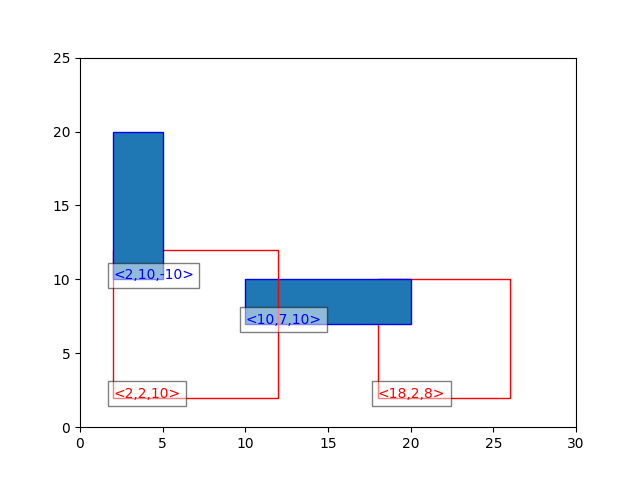
\includegraphics[width=0.65\textwidth]{images/ABGenome.png}
    \caption[All-Black example]{An example of a simple All-Black genome}
    \label{fig:all_black}
\end{figure}

\subsection{Grid-Graph genome}
\label{subsec:grid_graph}
\textit{Gird-Graph} was introduced by \citeauthor{bari_evolutionary-based_2023} with the aim of overcoming All-Black's problems.

The genome is similar to \textit{All-Black} in the sense that the map is initially full of walls and \textit{rooms} and \textit{corridors} are then placed on it. Given a map made of $H$ x $W$ tiles, Grid-Graph divides the map into an $R$ x $C$ grid where each cell occupies $r$ x $c$ tiles. 

Each cell can either contain one or no \textbf{room}, which is an axis aligned rectangle, defined by the width of the room $w$ (between 1 and $c$), the height of the room $h$ (between 1 and $r$) and the coordinates of the lower left corner of the room relative to the cell, so an $x$ (between 0 and $c$ - $w$ - 1) and a $y$ (between 0 and $r$ - $h$ - 1). Thus, the genome will contain an $R$ x $C$ matrix of rooms, where a room in cell ($i$, $j$) is defined with the above quartet of values, or a special value \textit{Nil} if no room is present in the cell.

Rooms can be connected by \textbf{corridors} if they are placed in horizontally or vertically adjacent cells. This is encoded in the genome via a single boolean value for each pair of horizontally or vertically adjacent cells, meaning that we have an $R$ x ($C$ - 1) matrix of boolean values for horizontal corridors, where the value in cell ($i$, $j$) indicates whether rooms in cell ($i$, $j$) and ($i$, $j$ + 1) are connected by a horizontal corridor, and a ($R$ - 1) x $C$ matrix of boolean values for vertical corridors, where the value in cell ($i$, $j$) indicates whether rooms in cell ($i$, $j$) and ($i$ + 1, $j$) are connected by a vertical corridor.

Similarly to \textit{All-Black}, the genome is converted to the phenotype by placing rooms and corridors on the map and keeping only the connected portion closest to the center of the map, eliminating all other unconnected regions. The genome supports mutation by randomly changing \textit{rooms} and \textit{corridors} and crossover by randomly exchanging \textit{rooms} and \textit{corridors} between two genomes.

\begin{figure}[hbt!]
    \centering
    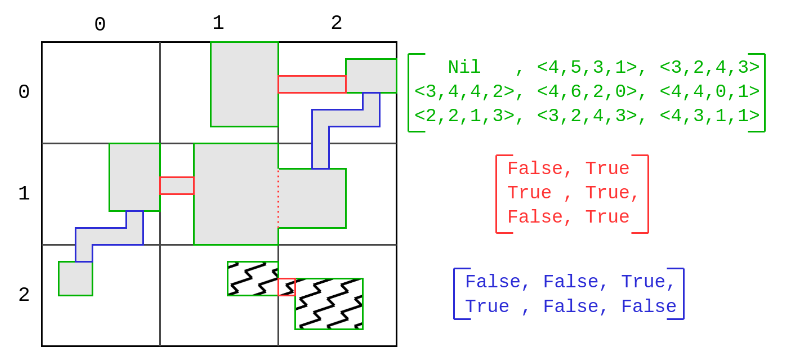
\includegraphics[width=0.85\textwidth]{images/GridGraph.png}
    \caption[Grid-Graph example]{An example of a simple Grid-Graph genome where rooms are shown in green, vertical corridors are shown in blue and horizontal corridors in red. Disconnected parts are filled with a zig-zagged line. Taken from \cite{bari_evolutionary-based_2023}.}
    \label{fig:grid_graph}
\end{figure}

\citeauthor{bari_evolutionary-based_2023} argues that \textit{Grid-Graph} overcomes the problems of \textit{All-Black}. The genome is more compact and less redundant, as rooms have no way to overlap. However, locality is still a problem (although in a more controlled way, since connected regions are separated only if their respective corridor is removed) and the resulting maps appear very simple, with the possible number of layouts being seemingly very limited.

\subsection{Point-Line genome}
\label{subsec:point_line}

We introduce in this work the \textit{Point-Line} genome, which takes its inspiration from \citet{olsted_interactive_2015}. The key idea that we borrow is that of defining explicitly the topology of the map by defining couples of points that are connected by L-shaped corridors.

Similarly to All-Black, the map is initially full of walls, and \textit{rooms} and \textit{corridors} are placed in it. 

The genome is defined as a list of $P$ \textbf{point couples}, where each point is defined by its $x$ and $y$ coordinates. Two points will be connected by an L-shaped corridor in the phenotype, and an additional value $c$ defines the orientation of the L-shaped corridor connecting the two: 0 indicates that, from the point that is leftmost and lower of the two, the corridor first extends horizontally and then vertically, while 1 indicates the opposite. Each point also serves as the coordinates for the center of an associated \textbf{room}, which is an axis aligned square of size $s$. The room is thus a square with each side being long $2s$. When the size is 0, no room is associated to the point.

The genome can be seen as a list of $P$ septets <$x_1$, $y_1$, $x_2$, $y_2$, $s_1$, $s_2$, $c$>, where the first four values are the coordinates of the two points, the next two are the size of the rooms associated to the points and the last is the orientation of the corridor connecting the two points. 

When the genome is converted to the phenotype, rooms are placed on the map and the corridors are drawn to connect the points. 

As already noted for the other representations, the resulting map may not be fully connected, which is similarly solved by keeping only the connected portion of the map that is closest to the center. The genome supports mutation by randomly changing the \textit{point couples}, the \textit{rooms} associated to the points or the orientation of the corridors, and crossover by randomly exchanging \textit{point couples} between two genomes.

We believe this genome to be capable of representing a wider range of topologies when compared to \textit{Grid-Graph}, while still being easily readable to the human player. Locality is improved with respect to \textit{All-Black} since rooms are explicitly connected by corridors, meaning that to remove a connection there needs to be a significant difference between the genomes, and simply moving a room also moves the corridor, keeping them connected. By coupling points and reusing coordinates between corridors and rooms, the genome is also more compact than \textit{All-Black}. We also believe that defining corridors by their start and end gives both long and short corridors an equal chance to appear, allowing \textit{Point-Line} to be more likely to explore different design, while long corridors in \textit{All-Black} are rarely found due to the need of placing a series of corridors to form a longer one.  However, the genome does not solve the problem of redundancy, as rooms can still overlap. This solution thus places itself in a sort of middle ground between \textit{All-Black} and \textit{Grid-Graph}, with the aim of combining the best of both.

\begin{figure}[hbt!]
    \centering
    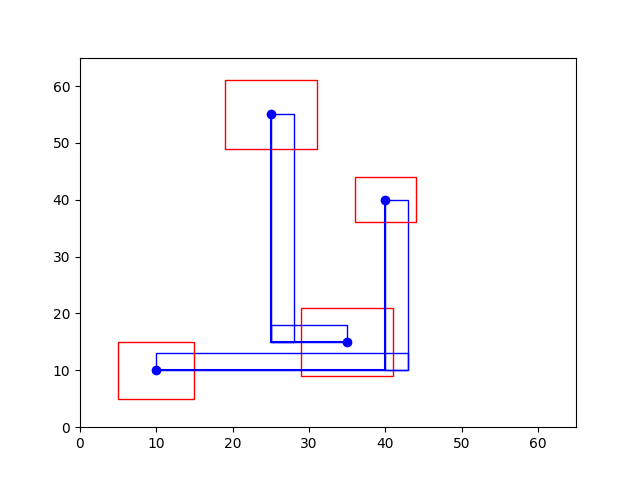
\includegraphics[width=0.65\textwidth]{images/PointGenome.png}
    \caption[Point-Line example]{An example of a simple Point-Line genome where points, L-shaped connections and related corridors raw shown in blue and rooms are shown in red.}
    \label{fig:point_line}
\end{figure}

\subsection{SMT-Genome}
\label{subsec:smt_genome}

We also introduce in this work the \textit{SMT-Genome}, which is inspired by \citet{whitehead_spatial_2020}. In their work, they propose to use a satisfiability modulo theories (SMT) solver\footnote{Satisfiability modulo theories is the field concerned with the satisfiability of mathematical formulas involving real numbers and complex data structures. An SMT solver is a tool that tries to determine said satisfiability.} to place rooms of varying dimension in a 2D map. 

Similarly to all other genomes we have discussed, the map is initially full of walls, and \textit{rooms} and \textit{corridors} are placed in it.
The genome is defined by a list of $R$ axis-aligned rectangular \textbf{rooms}, where each room is defined only by its width and height, and a list of $L$ \textbf{lines}, which are defined by two points in the 2D maps that are logically connected by a line, forming a segment. Finally, the genome also includes a parameter for minimum separation, $s$, which determines the minimum distance between rooms' borders. 

The genome is thus a list of $R$ + $L$ + 1 elements, where the first $R$ elements are couples of values representing rooms, the following $L$ are quadruplets with the coordinates of the two points of the line and the last is the minimum separation.

Differently from the other genomes, rooms are not encoded with their position, as their position is determined by the SMT solver. Thus, when the genome needs to be converted to a phenotype, a position has to be found for each room. This is done following an approach similar to that of \citet{whitehead_spatial_2020}; a number of linear constraints\footnote{Expressions where all the terms are of the first order, thus no exponents, logarithms, etc. appear.} are defined where the terms are the $x$ and $y$ coordinates of each room's upper left corner. We then used Pythons \textit{Z3}\footnote{\url{https://pypi.org/project/z3-solver/}} library to solve the system of constraints, which returns the coordinates of the upper left corner of each room.

The first class of constraints ensures that all rooms are placed inside the map's border. 
\begin{equation}
    \begin{split}
            \forall r_i \in Rooms,\: x_{r_i} >= 0 \land x_{r_i} <= width_{map} - width_{r_i} \\ \land y_{r_i} >= 0 \land y_{r_i} <= height_{map} - height_{r_i}
    \end{split}
\end{equation}

The second ensures that no two rooms overlap.

\begin{equation}
\label{eq:room_overlap}
    \begin{split}
        \forall r_i, r_j \in Rooms\, \mid\,  r_i != r_j, \\
        y_{r_j} <= y_{r_i} - height_{r_j} - s\: \lor \\
        y_{r_i} <= y_{r_j} - height_{r_i} - s\: \lor \\
        x_{r_j} <= x_{r_i} - width_{r_j} - s\: \lor \\
        x_{r_i} <= x_{r_j} - width_{r_i} - s
    \end{split}
\end{equation}

The equation \cref{eq:room_overlap} ensures that no two rooms overlap by asserting, in order, that the room $j$ must be located either fully above, below, to the left or to the right of room $i$, at a distance of at least $s$.

The last class of constraints ensures that rooms are placed close to the lines defined by the genome. To achieve this, lines are associated to a static common parameter called $linewidth$ and their $slope$ is calculated. We must note that Z3 requires integer coefficients, so many interesting slopes between 0 and 1 would be truncated; to solve this, the vertical $y$ dimension is scaled up by a factor of 1000, and then de-scaled at the end. The constraints are defined as follows:

\begin{equation}
\label{eq:room_line}
    \begin{split}
        &\forall l_i \in Lines,\, \forall r_j \in Rooms, \\
        &y_{r_j} \leq slope_{l_i} * (x_{r_j} - x_{end_{l_i}} + linewidth) + y_{end_{l_i}} \:\land \\
        &y_{r_j} \geq slope_{l_i} * (x_{r_j} - x_{end_{l_i}} - linewidth + width_{r_j}) + y_{end_{l_i}}
    \end{split}
\end{equation}

\textit{Z3} will solve all these constraints and return the coordinates of the upper left corner of each room, if one such solution exists.

Once the rooms' positions are defined, rooms must be connected using corridors. Similarly to \citeauthor{whitehead_spatial_2020}, first we define connections between two rooms by drawing a Delaunay triangulation\footnote{A type of triangulation (which is the subdivision of a planar object into triangles) which ensures that, for a set of points, that no circumcircle (circle passing through a triangle's vertices) contains any other point.} with the rooms' positions, obtaining a graph where an edge represents that the two rooms are connected by a corridor. Subsequently, we only keep a subset of connections by drawing a minimum spanning tree (MST)\footnote{A tree that connects all the vertices of a graph with the minimum possible total edge length.} on the triangulation, ensuring that we keep a connected graph. Rooms that are connected by an edge in the MST are then connected physically by a corridor in the phenotype. Corridors are built following a deterministic procedure, based on the rooms' relative positions, to avoid introducing another layer of randomness. 

We noted that the maps generated via this method were not sufficiently connected; \citeauthor{whitehead_spatial_2020} was interested in dungeon designs, where an SMT could suitably represent a linear layout with a start, an end and some optional rooms and paths, but multiplayer FPS maps require more complex topologies that entail loops, arenas and alternate routes, as discussed in \cref{sec:level_design}. We thus decided to add connections between rooms via a heuristic; given a line, rooms that are intersected by it are connected by a corridor, if they weren't already connected.

\begin{figure}[hbt!]
    \centering
    \subfloat[Example of a simple SMT-Genome without added corridors]{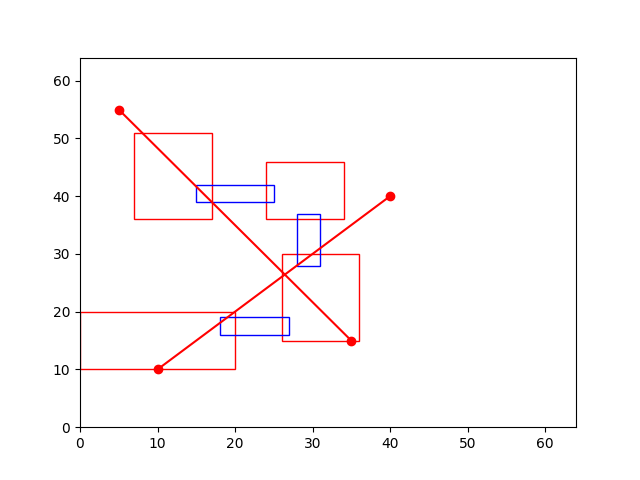
\includegraphics[width=0.45\textwidth]{images/SMT_NotAdded.png}}
    \qquad
    \subfloat[Example of a simple SMT-Genome with added corridors]{\includegraphics[width=0.45\textwidth]{images/SMT_added.png}}
    \caption[SMT-Genome lines]{An example of how corridors are added between rooms intersected by a line.}
    \label{fig:smt_genome}
\end{figure}

The genome supports mutation by randomly changing the rooms and lines and crossover by randomly exchanging rooms and lines between two genomes.

It must be noted that, differently from the other genomes, the SMT-Genome is not deterministic; while we can set a seed in \textit{Z3}, the result of the solving process may still vary when run on the same genome due to the nature of the solver itself. This could be a problem as it could lead to poor locality. Genomes may also have no feasible solution, in which case we are forced to discard it.

\begin{figure}[hbt!]
    \centering
    \subfloat{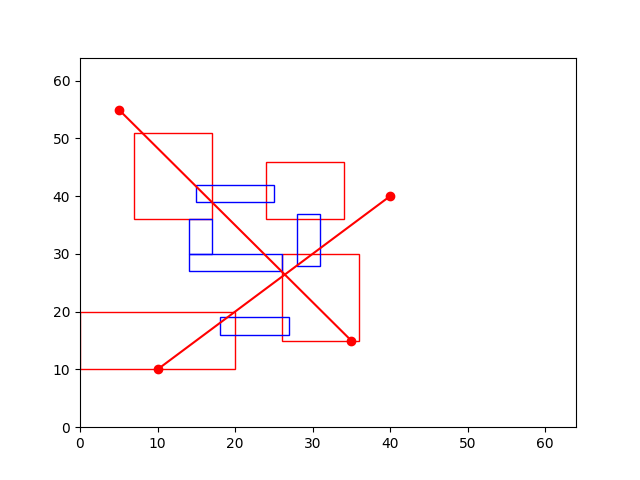
\includegraphics[width=0.45\textwidth]{images/SMT_Added.png}}
    \qquad
    \subfloat{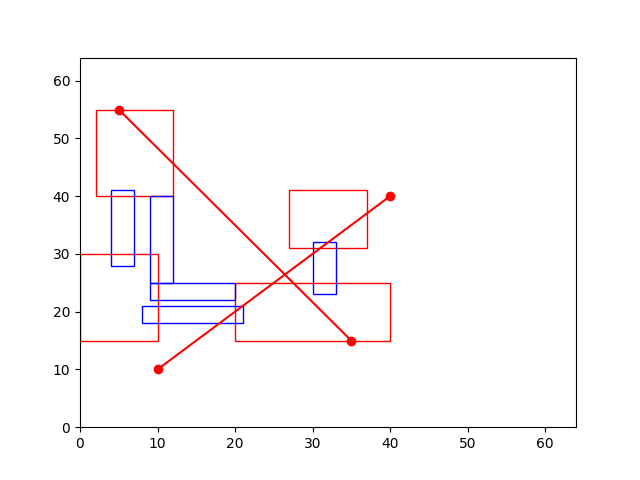
\includegraphics[width=0.45\textwidth]{images/SMT_Added_2.png}}
    \caption[SMT-Genome determinism]{Examples of how the same SMT genome may lead to different results.}
    \label{fig:smt_genome_determinism}
\end{figure}

\subsection{Common Areas-Phenotype}
All genomes are transformed to a common phenotype, called \textbf{Areas-Phenotype}. This phenotype is then supplied to \textit{Project Arena} where it is transformed into the internal textual representation used to build the actual map. This phenotype describes the map as rectangles of walkable tiles placed on a grid where each tile is a wall.

The \textit{Areas-Phenotype} is an object which contains:

\begin{itemize}
    \item \textit{MapWidth}: The map's width
    \item \textit{MapHeight}: The map's height
    \item \textit{MapScale}: The scale of the map, used by the framework to enlarge or shrink the map's size.
    \item \textit{Areas}: A list of areas, where each area is a rectangle full of walkable spaces defined by:
    \begin{itemize}
        \item \textit{BottomRow}: The $y$ coordinate of the bottom row of the area
        \item \textit{TopRow}: The $y$ coordinate of the top row of the area
        \item \textit{LeftCol}: The $x$ coordinate of the left column of the area
        \item \textit{RightCol}: The $x$ coordinate of the right column of the area
        \item \textit{IsCorridor}: A boolean value indicating whether the area is a corridor or a room
    \end{itemize}
\end{itemize}

\clearpage
\section{Features}
\label{sec:features}
To accomplish our goal, we tried to define a variety of different features that could describe a map from. We identified two main categories of features:  \textit{emergent} and \textit{topological}.

\subsection{Emergent features}
\label{subsec:emergent_features}
We define \textbf{emergent} features as those that "emerge" from actual gameplay and that are not directly tied to the map's topological features, such as the number of kills. The map's layout will surely influence the result of the match, but we cannot predict emergent features solely from the map's topology, and instead we must rely on simulations to gather them.

These features utilize the metrics defined in \cref{subsec:pa_data_gathering} and are defined as follows:
\begin{itemize}
    \item \textit{entropy}: A measure used to infer the map's balance, calculated as follows:
    \begin{equation}
        entropy = \sum_{i=1}^{n} - \left(\dfrac{k_i}{k_{tot}}\right) \log_2 \left(\dfrac{k_i}{k_{tot}}\right)
    \end{equation}
    Where for each bot $i$ the number of kills $k_i$ is divided by the total number of kills $k_{tot}$ and multiplied by the logarithm of the result, and the entropy is then the sum of these values. Possible values range from 0 to 1, with 1 representing a balanced match and 0 meaning a wildly unbalanced match.
    \item \textit{ratio}: The ratio of the number of kills to the number of deaths.
    \item \textit{pace}: The frequency of combat engagements normalized between 0 and 1, calculated as follows:
    \begin{equation}
        pace = 2 * \dfrac{1}{1 + \exp \left(-5 * \dfrac{NumberOfFights}{\sum TimeToEngage}\right)} - 1
    \end{equation}
    This sigmoid function computes values close to 0.9 when the average time to engage is 3 seconds.
    \item \textit{fightTime}: The average time the bots spend exclusively fighting, calculated as follows for $N$ bots:
    \begin{equation}
        fightTime = \dfrac{  \sum_{i}^{N} \left(timeInFight_i - timeBetweenSights_i - timeToSurrender_i\right) }{ N * gameLength}
    \end{equation}
    \item \textit{pursueTime}: The average time the bots spend pursuing an enemy, which include the time spent looking for it, calculated as follows for $N$ bots:
    \begin{equation}
        pursueTime = \dfrac{  \sum_{i}^{N} \left(timeInFight_i\right) }{ N * gameLength}
    \end{equation}
    \item \textit{sightLossRate}: The average time between losing sight of an enemy and detecting it again, calculated as follows for $N$ bots:
    \begin{equation}
        sightLossRate = \dfrac{  \sum_{i}^{N} timeBetweenSights_i }{ \sum_{i}^{N} timeInFight_i}
    \end{equation}
    \item \textit{targetLossRate}: The number of retreats compared to the number of fights, calculated as follows for $N$ bots:
    \begin{equation}
        targetLossRate = \dfrac{  \sum_{i}^{N} numberOfRetreats_i }{ \sum_{i}^{N} numberOfFights_i}
    \end{equation}
    \item \textit{killDiff}: The difference between the number of kills and the number of deaths.
\end{itemize}

Besides these, we also define some features leveraging the data gathered by the framework, particularly the raw data about kill's positions, death's positions and bots' positions (sampled at a fixed interval of 0.5s) during the match. For each bot, we plot each position on a discretized grid representing the map, obtaining a heatmap of the positions of the kills and deaths. We then apply a Gaussian filter to the heatmap to smooth it, and calculate the following features on each of the three heatmaps:

\begin{itemize}
    \item \textit{maxValue}: The maximum value of the heatmap.
    \item \textit{averageLocalMaximaValue}: The average of the values of all local maxima of the heatmap.
    \item \textit{stdLocalMaximaValue}: The standard deviation of the values of all local maxima.
    \item \textit{quantile25}: The first quartile of the heatmap's values.
    \item \textit{quantile50}: The second quartile (median) of the heatmap's values.
    \item \textit{quantile75}: The third quartile of the heatmap's values.
    \item \textit{localMaximaNumber}: The number of local maxima of the heatmap.
    \item \textit{localMaximaTopDistance}: The distance between the two local maxima with the highest values.
    \item \textit{localMaximaAverageDistance}: The average distance between all local maxima.
    \item \textit{coverage}: The percentage of the walkable map covered by the heatmap, meaning that the value is not 0 in that position.
\end{itemize}

\begin{figure}[hbt!]
\label{fig:heatmaps_example}
    \centering
    \subfloat{{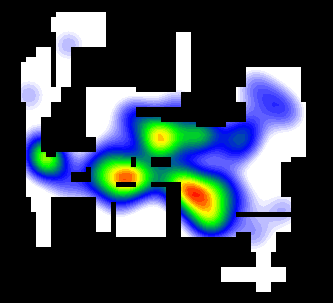
\includegraphics[width=0.4\textwidth]{images/Deaths_Heat_Example.png} }}
    \qquad
    \subfloat{{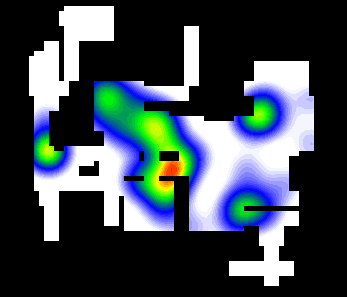
\includegraphics[width=0.4\textwidth]{images/Kill_Heat_Example.png} }}
    \caption[Heatmaps example]{An example of a heatmap of the deaths' positions (left) and the kills' positions (right)}
\end{figure}

We also utilize the kills and deaths' positions to calculate the "kill traces". A kill trace is the path of the bullet that killed a bot, and we can obtain them by connecting the position of the killer to the position of the killed bot. We then calculate the following features on the kill traces:

\begin{itemize}
    \item \textit{maxTraces}: The longest kill trace.
    \item \textit{averageTraces}: The average length of the kill traces.
    \item \textit{quantile25Traces}: The first quartile of the kill traces' lengths.
    \item \textit{quantile50Traces}: The second quartile (median) of the kill traces' lengths.
    \item \textit{quantile75Traces}: The third quartile of the kill traces' lengths.
\end{itemize}

\begin{figure}[hbt!]
\label{fig:kill_traces_example}
    \centering
    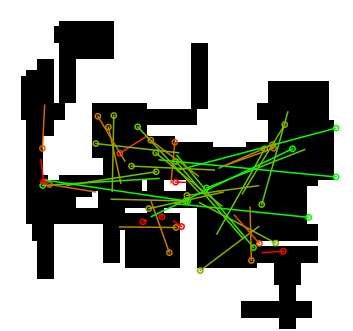
\includegraphics[width=0.4\textwidth]{images/Traces_Example.png}
    \caption[Kill traces example]{An example of the kill traces over a match, with the killer bot's position marked with a circle and brighter colors indicating longer traces.}
\end{figure}

\subsection{Topological features}
\label{subsec:topological_features}
Topological features are those that describe the map's topology, and they can be directly inferred from the map itself without the need of simulations. The simplest example is the following feature: 

\begin{itemize}
    \item \textit{area}: The number of tiles that are walkable compared to the total number of tiles in the map.
\end{itemize}

In order to extract interesting topological features it was clear that the map's representations as matrices of tiles would not be directly suitable, so we decided to convert the map to a graph representation with the aim of identifying rooms as nodes and add edges between rooms that are directly connected by a corridor. To achieve this goal, we looked at two methods for room segmentation. 

The first is the "Distance Transform-based Segmentation" approach used in \citep{bormann_room_2016}. First, we compute the Euclidean distance transform\footnote{\raggedright\url{https://docs.scipy.org/doc/scipy-0.14.0/reference/generated/scipy.ndimage.morphology.distance_transform_edt.html}} on the map, which is represented as a grid of tiles that are either walkable or walls, obtaining a map of distances. Then we locate the local maxima that are at least 3 tiles apart. These points serve as the room center coordinates that are used as markers for a Watershed\footnote{\raggedright\url{https://scikit-image.org/docs/stable/api/skimage.segmentation.html\#skimage.segmentation.watershed}} algorithm, using the negative distance map as basin. The identified rooms are then used as nodes to build the graph, where edges are added between rooms with common borders. Figure \cref{fig:dt_segmentation} shows an example of the result.

\begin{figure}[H]
    \centering
    \subfloat[The rooms identified by the algorithm]{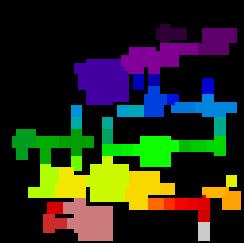
\includegraphics[height=0.4\textwidth]{images/graph_dist_color.png}}
    \qquad
    \subfloat[The graph obtained connecting adjacent rooms]{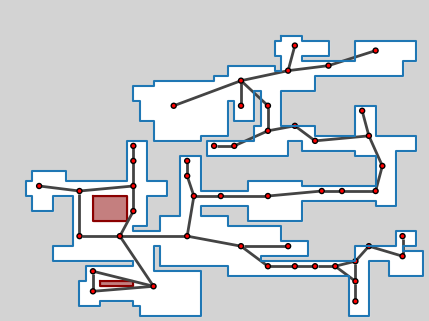
\includegraphics[height=0.4\textwidth]{images/graph_dist.png}}
    \caption[Distance Transform Segmentation example]{An example of the Distance Transform-based Segmentation}
    \label{fig:dt_segmentation}
\end{figure}

The second is the approach for region decomposition based on line segment Voronoi diagrams detailed by \citet{perkins_terrain_2010}, which we will describe here briefly. Starting from a map represented by a grid of walkable or wall tiles, we use a flood fill algorithm to identify the external wall (which we ensure is always a single polygon by adding a wall border to the map) and all obstacles (contiguous areas of walls inside a walkable part of the map) and transform them into polygons. Then we create a Voronoi diagram\footnote{\raggedright\url{https://pypi.org/project/pyvoronoi/}} of the line segments of the polygons, removing from the diagram secondary edges and edges inside the obstacles' polygons. The Voronoi diagram is transformed then into a graph, and for each node we compute a \textit{radius}, defined as the minimum distance from the node to the nearest obstacle. We use this radius to prune the graph by iteratively removing leaves whose radius is smaller than their parent's. Then we identify \textit{regions} (\textit{rooms}, in our case) and \textit{chokepoints} based on the degree of a node and its radius and, to simplify the graph, we merge adjacent rooms using some heuristics. The process and its results are shown in figure \cref{fig:voronoi_region_decomposition}.

\begin{figure}[hbt!]
    \centering
    \subfloat[The map as a grid.]{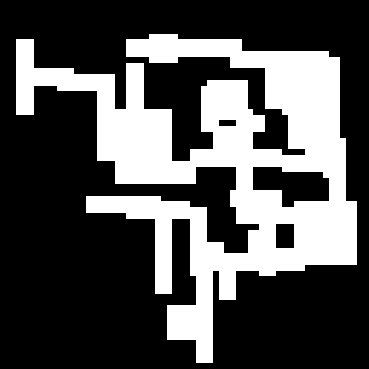
\includegraphics[height=0.3\textwidth]{images/graph_v_1.png}}
    \qquad
    \subfloat[The map represented by polygons.]{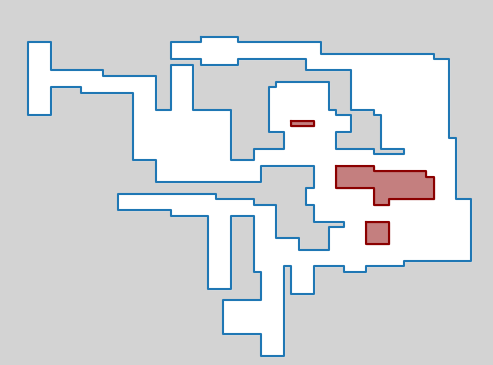
\includegraphics[height=0.3\textwidth]{images/graph_v_2.png}}
    \qquad
    \subfloat[The line segment Voronoi diagram.]{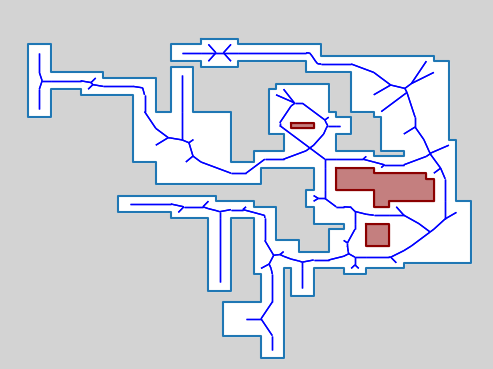
\includegraphics[height=0.3\textwidth]{images/graph_v_3.png}}
    \qquad
    \subfloat[The graph obtained by the diagram after pruning.]{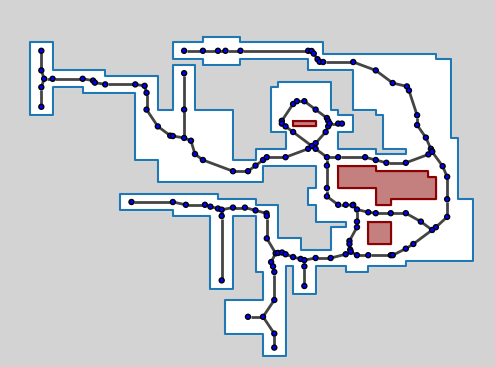
\includegraphics[height=0.3\textwidth]{images/graph_v_4.png}}
    \qquad
    \subfloat[Rooms (red) and chokepoints (yellow) identification.]{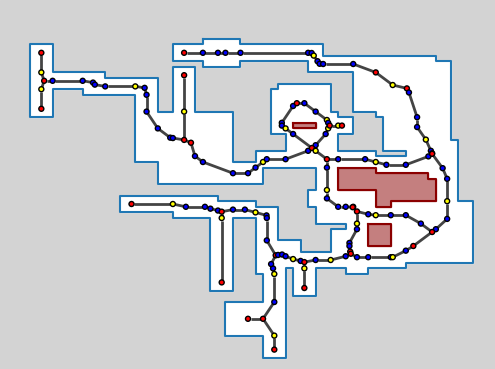
\includegraphics[height=0.3\textwidth]{images/graph_v_5.png}}
    \qquad
    \subfloat[The final graph after rooms are heuristically merged.]{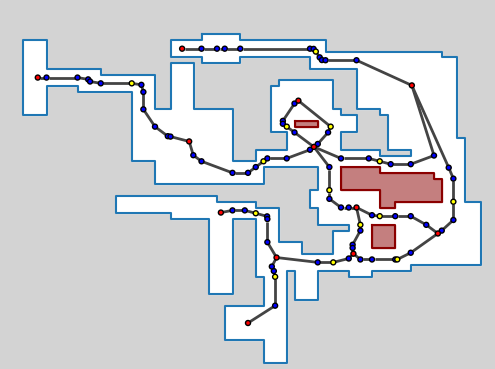
\includegraphics[height=0.3\textwidth]{images/graph_v_6.png}}
    
    \caption[Voronoi Region Decomposition example]{An example of the Voronoi Region Decomposition process.}
    \label{fig:voronoi_region_decomposition}
\end{figure}

While results are similar, the Voronoi-based approach felt more suited to our needs, providing a graph that structurally resembles the map's topology and distinguishes relevantly between rooms and corridors. Moreover, the Distance Transform-based approach is often unable to identify multiple connections between two rooms, which is a common and important feature of FPS maps. In figure \cref{fig:graph_comparison} we show a comparison to facilitate the understanding of the problem at hand.

\begin{figure}[hbt!]
    \centering
    \subfloat[Distance Transform-based Segmentation]{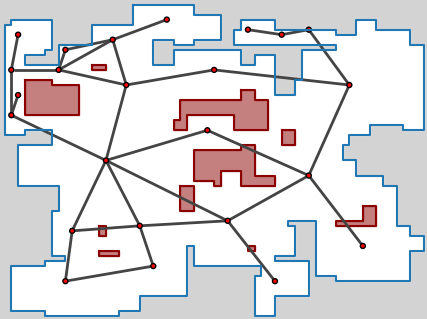
\includegraphics[width=0.45\textwidth]{images/graph_compare_dist.png}}
    \qquad
    \subfloat[Voronoi Region Decomposition]{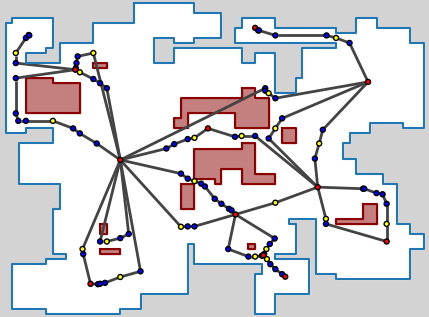
\includegraphics[width=0.45\textwidth]{images/graph_compare_vor.png}}
    \caption[Graph comparison]{A comparison between the graphs obtained with the two methods. Notice how in the bottom-right corner of the left image the two rooms only have a single edge connecting them, while in the right image they have two.}
    \label{fig:graph_comparison}
\end{figure}

Leveraging this graph, we defined features that we believed to be relevant in order to describe and distinguish different FPS maps, such as loops, alternate routes and other concepts discussed in \cref{sec:level_design}.
Thus, for each map we extract the following \textbf{graph-based} features:

\begin{itemize}
    \item \textit{roomNumber}: The number of nodes that represent rooms in the graph.
    \item \textit{averageRoomMinDistance}: The average minimum distance between rooms, computed with the shortest path algorithm.
    \item \textit{stdRoomMinDistance}: The standard deviation of the minimum distance between rooms.
    \item \textit{averageRoomRadius}: The average radius of the rooms, computed as the minimum distance from the room's node to the nearest obstacle.
    \item \textit{stdRoomRadius}: The standard deviation of the rooms' radius.
    \item \textit{averageRoomBetweenness}: The average betweenness centrality of the rooms' nodes, which is based on the number of the shortest paths that pass through the room.
    \item \textit{stdRoomBetweenness}: The standard deviation of the rooms' betweenness centrality.
    \item \textit{averageRoomCloseness}: The average closeness centrality of the rooms' nodes, which based on the inverse of the sum of the shortest paths from the room to all other rooms.
    \item \textit{stdRoomCloseness}: The standard deviation of the rooms' closeness centrality.
    \item \textit{averageMincut}: The average value of the minimum cut between every couple of distinct rooms, which is the minimum number of edges that must be removed to disconnect the two rooms. 
    \item \textit{stdMincut}: The standard deviation of the minimum cut.
    \item \textit{maxMincut}: The minimum cut with the highest value.
    \item \textit{minMincut}: The minimum cut with the lowest value.
    \item \textit{averageEccentricity}: The average eccentricity of the rooms' nodes, which is the maximum distance from the room to all other rooms.
    \item \textit{stdEccentricity}: The standard deviation of the rooms' eccentricity.
    \item \textit{diameter}: The diameter of the graph, which is the maximum eccentricity.
    \item \textit{radius}: The radius of the graph, which is the minimum eccentricity.
    \item \textit{periphery}: The number of rooms that are in the periphery of the graph, which are the rooms with eccentricity equal to the diameter. In our case, since we use floating point distances, we heuristically consider rooms with eccentricity within 2 tiles of the diameter.
    \item \textit{center}: The number of rooms that are in the center of the graph, which are the rooms with eccentricity equal to the radius. In our case, since we use floating point distances, we heuristically consider rooms with eccentricity within 2 tiles of the radius.
    \item \textit{peripheryPercent}: The percentage of rooms that are in the periphery.
    \item \textit{centerPercent}: The percentage of rooms that are in the center.
    \item \textit{density}: The density of the graph, which is the ratio of the number of edges to the number of possible edges.
    \item \textit{numberCyclesOneRoom}: The number of fundamental cycles that contain at least one room.
    \item \textit{averageLengthCyclesOneRoom}: The average length of the cycles that contain at least one room.
    \item \textit{stdLengthCyclesOneRoom}: The standard deviation of the length of the cycles that contain at least one room.
    \item \textit{numberCyclesTwoRooms}: The number of fundamental cycles that contain at least two rooms.
    \item \textit{averageLengthCyclesTwoRooms}:  The average length of the cycles that contain at least two rooms.
    \item \textit{stdLengthCyclesTwoRooms}: The standard deviation of the length of the cycles that contain at least two rooms.
\end{itemize}

We also believe that another important component of a map's topology is the \textit{visibility} of the maps; maps in FPS games may reward certain play-styles depending on how far away a player can see from any point (e.g. a big arena with no obstacles will always favor long-ranged weapons), and designers alternate between open and closed spaces to avoid favoring a single play-style. Having observed that, we define the visibility of a walkable tile in a map as the number of walkable tiles that are visible from it. To compute the visibility, we build the \textit{visibility graph}; each walkable tile is a node, and for each tile we run the DDA algorithm\footnote{Digital Differential Analyzer is an algorithm for line generation, typically used in computer graphics, to draw lines on a grid from a starting tile (or pixel) to an ending one.} to all other walkable tiles. If no wall is in the path, we add an edge between the two nodes. Then, the resulting graph can be converted to a \textit{visibility matrix} by assigning to each tile the number of nodes to which it is connected.

While this naive approach works, the algorithm is $O\left(N^{2}\right)$ and even after careful optimization takes upwards of 40 seconds to compute the visibility of larger maps. For this reason, we opted for the faster, approximate approach of Grid-Based visibility \cite{goldstein_quick_2023}, in which we loop over every tile of the map and perform a linear interpolation on the whole map. The result can be computed in under a second for all tested maps and the visibility matrix is a good approximation of the true visibility, although the number of tiles visible from any tile is generally lower than with the naive method (see figure \cref{fig:visibility_example}).

\begin{figure}[hbt!]
    \centering
    \subfloat[Naive method, computed in 28.77s]{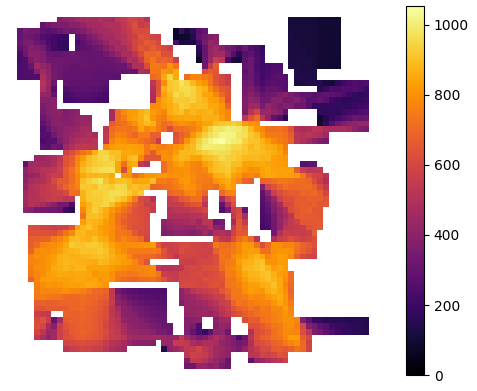
\includegraphics[width=0.45\textwidth]{images/visibility_old.png}}
    \qquad
    \subfloat[The visibility matrix, computed in 0.26s]{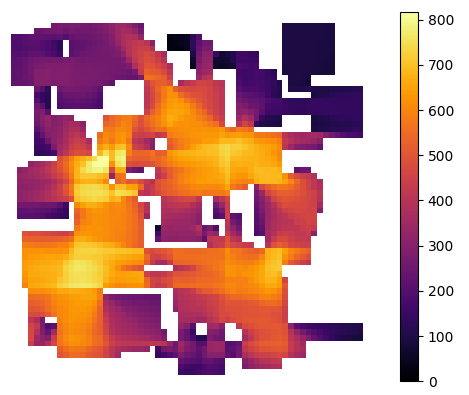
\includegraphics[width=0.45\textwidth]{images/visibility_new.png}}
    \caption[Visibility comparison]{Examples of the visibility matrix obtained with the naive method and the grid-based method. The color of a tile represents the number of tiles visible from it.}
    \label{fig:visibility_example}
\end{figure}

From this visibility matrix we can extract the following \textbf{visibility-based} features:

\begin{itemize}
    \item \textit{maxValueVisibility}: Maximum value of the visibility matrix, which represents the maximum number of tiles visible from a single tile.
    \item \textit{maxValuePercentVisibility}: Maximum value of the visibility matrix divided by the total number of walkable tiles.
    \item \textit{averageLocalMaximaValuePercentVisibility}: The average of the values of all local maxima of the visibility matrix divided by the total number of walkable tiles.
    \item \textit{averageValuePercentVisibility}: The average value of the visibility matrix divided by the total number of walkable tiles.
    \item \textit{quantile25PercentVisibility}: The first quartile of the visibility matrix divided by the total number of walkable tiles.
    \item \textit{quantile50PercentVisibility}: The second quartile (median) of the visibility matrix divided by the total number of walkable tiles.
    \item \textit{quantile75PercentVisibility}: The third quartile of the visibility matrix divided by the total number of walkable tiles.
    \item \textit{stdValuePercentVisibility}: The standard deviation of the values of the visibility matrix divided by the total number of walkable tiles.
    \item \textit{localMaximaNumberVisibility}: The number of local maxima of the visibility matrix.
    \item \textit{localMaximaTopDistanceVisibility}: The distance between the two local maxima with the highest values of the visibility matrix.
    \item \textit{localMaximaAverageDistanceVisibility}: The average distance between all local maxima of the visibility matrix.
    \item \textit{stdLocalMaximaValuePercentVisibility}: The standard deviation of the values of all local maxima of the visibility matrix divided by the total number of walkable tiles.
\end{itemize}

Another particularly interesting topological measure is a map's symmetry. Symmetry is an important concept in level design, both from a balancing perspective and from an aesthetic perspective. We have measured symmetry as the percentage of tiles that are equal to their symmetrical counterpart with respect to the map's center axis, obtaining the following \textbf{symmetry-based} features:

\begin{itemize}
    \item \textit{xSymmetry}: The percentage of tiles that are equal to their symmetrical counterpart with respect to the map's vertical axis.
    \item \textit{ySymmetry}: The percentage of tiles that are equal to their symmetrical counterpart with respect to the map's horizontal axis.
    \item \textit{maxSymmetry}: The maximum value between xSymmetry and ySymmetry.
\end{itemize}

Finally, we have tried to define measures that would describe certain types of maps that could be interesting to illuminate. We have thus defined the following \textbf{aggregate} features:

\begin{itemize}
    \item \textit{balanceTopology}: A measure of how balanced a map's topology is, meaning that rooms are well-connected, loops are present, and rooms are generally well-distributed. It is calculated as follows:
    \begin{equation}
    \begin{split}
        &explorationFactor = clip\left(\dfrac{averageMincut}{2}, 0, 1\right) \\
        &evenlySpacedFactor = 1 - \dfrac{stdRoomMinDistance}{30} \\
        &cyclesFactor = clip\left(\dfrac{numberCyclesTwoRoom}{5}, 0, 1\right) \\
        &balanceTopology = explorationFactor + evenlySpacedFactor \\
        &+ cyclesFactor
    \end{split}
    \end{equation}
    Note that the value "30" in the evenlySpacedFactor is an empirical value from the observed maximum of \textit{stdRoomMinDistance}.
    \item \textit{explorationPlusVisibility}: A measure to describe how much a map encourages exploration by being well-connected and having good visibility. It is calculated as follows:
    \begin{equation}
    \begin{split}
        &explorationFactor = clip\left(\dfrac{averageMincut}{2}, 0, 1\right) \\
        &visibilityFactor = clip\left(localMaximaNumberVisibility, 0, 1\right)\\ 
        &* averageValuePercentVisibility \\
        &explorationPlusVisibility = explorationFactor + visibilityFactor
    \end{split}
    \end{equation}
\end{itemize}

\section{Summary}
In this chapter we have described the already existing genomes \textit{All-Black} and \textit{Grid-Graph}, and the newly defined genomes \textit{Point-Line} and \textit{SMT-Genome}. We have also described the common phenotype \textit{Areas-Phenotype} used to interface the representations with \textit{Project-Arena}. We have then listed and described all the emergent features extracted from simulated gameplay data and all the topological features extracted from the map's topology, using room segmentation to derive a graph representation and graph-based visibility methods to extract the visibility matrix.